\chapter{Zeitaufgelöste Simulation}
\begin{mybox}
	\textbf{Aufgabe 1. :}	Formulieren Sie das System in der Form $ u' = F(t,u) $
\end{mybox}

Die Randbedingungen

\begin{equation}
	D\cdot \frac{\partial u}{\partial z}(0)=S_Lu(0),\quad D\frac{\partial u}{\partial z}(d)=-S_Ru(d)
\end{equation}

und:

\begin{align*}
	&k=k_1+k_2\cdot N_D\\
	&s_i=s(z_i)\\
	&h=\frac{d}{N}\\
	&u(i)\approx u_i
\end{align*}

Analog wie im zweiten Abschnitt

\begin{equation}
	u' =\frac{u_{i+1} -u_{i-1}}{2h}
\end{equation}

\begin{equation}
	u''=\frac{u_{i+1} -{2u}_i +u_{i-1} }{h^2 }
\end{equation}

Anschließend werden die Ableitungen jeweils in die Gleichung sowie Randbedingungen eingesetzt:

\begin{equation}
	u'_i\left(t\right)=D\frac{u_{i+1} \left(t\right)-{2u}_i \left(t\right)+u_{i-1} \left(t\right)}{h^2 }-\left(k_1 +k_2 N_D \right)u\left(t\right)-k_2 u^2 \left(t\right)+s_i \left(t,z_i \right)
\end{equation}

Dann setzt man die Randbedingungen in die Gleichung für $ i = 0 $ und $ i = N $ ein:

\begin{equation}
	u^{\prime } \left(t,z_i \right)=D\frac{u_{i+1} \left(t\right)-{2u}_i \left(t\right)+u_{i-1} \left(t\right)}{h^2 }-ku_i \left(t\right)-k_2 {u_i }^2 \left(t\right)+s_i \left(t,z\right)
\end{equation}

für $ i = 0 $ gilt:

\begin{equation}
	u^{\prime } \left(t{,z}_i \right)=D\frac{u_1 \left(t\right)-{2u}_0 \left(t\right)+u_{-1} \left(t\right)}{h^2 }-ku_0 \left(t\right)-k_2 {u_0 }^2 \left(t\right)+s_0 \left(t,z\right)
\end{equation}

\begin{equation}
u^{\prime } \left(t{,z}_i \right)=D\frac{u_1 -{2u}_0 +u_1 -\frac{S_L \cdot 2h}{D}u_0 }{h^2 }-ku_0 -k_2 {u_0 }^2 +s_0 \left(z\right)	
\end{equation}

\begin{equation}
	u^{\prime } \left(t{,z}_i \right)=D\frac{2u_1 -{2u}_0 -\frac{S_L \cdot 2h}{D}u_0 }{h^2 }-ku_0 -k_2 {u_0 }^2 +s_0 \left(z\right)
\end{equation}

\begin{equation}
	u^{\prime } \left(t{,z}_i \right)=\frac{2{Du}_1 }{h^2 }-\frac{2{Du}_0 }{h^2 }-\frac{D\cdot S_L 2{hu}_0 }{D\cdot h^2 }-ku_0 -k_2 {u_0 }^2 +s_0 \left(z\right)
\end{equation}

\begin{equation}
	u^{\prime } \left(t{,z}_i \right)=\frac{2{Du}_1 }{h^2 }-\frac{2{Du}_0 }{h^2 }-\frac{S_L 2u_0 }{h}-ku_0 -k_2 {u_0 }^2 +s_0 \left(z\right)
\end{equation}

\begin{equation}
	u^{\prime } \left(t{,z}_i \right)=u_0 \left(t\right)\left(-\frac{2D}{h^2 }-\frac{{2S}_L }{h}\;-k-k_2 u_0 \left(t\right)\right)+u_1 \left(t\right)\left(\frac{2D}{h^2 }\right)+s_0 \left(t,z_0 \right)
\end{equation}


für $ i = N $ gilt:

\begin{equation}
	u^{\prime } \left(t{,z}_i \right)=D\frac{u_{N+1} \left(t\right)-{2u}_N \left(t\right)+u_{N-1} \left(t\right)}{h^2 }-ku_N \left(t\right)-k_2 {u_N }^2 \left(t\right)+s_N \left(z_N \right)
\end{equation}


\begin{equation}
	u^{\prime } \left(t{,z}_i \right)=D\frac{u_{N-1} -\frac{\;S_R \cdot 2h}{D}\cdot u_N -{2u}_N \left(t\right)+u_{N-1} \left(t\right)}{h^2 }-ku_N \left(t\right)-k_2 {u_N }^2 \left(t\right)+s_N \left(z_N \right)	
\end{equation}
	
	
\begin{equation}
	u^{\prime } \left(t{,z}_i \right)=u_N \left(t\right)\left(-\frac{\;2S_R }{h}-\frac{\;2D}{h^2 }-k-k_2 u_N \left(t\right)\right)+u_{N-1} \left(t\right)\left(\frac{2D}{h^2 }\right)+s_0 \left(t,z_N \right)	
\end{equation}

Somit kann unsere Gleichung aufgestellt werden:

\begin{equation}
		F(t,u)= 
\begin{bmatrix}
	\begin{array}{c}
		u_0 \left(t\right)\left(-\frac{2D}{h^2 }-\frac{{2S}_L }{h}\;-k-k_2 u_0 \left(t\right)\right)+u_1 \left(t\right)\left(\frac{2D}{h^2 }\right)+s_0 \left(t,z_0 \right)\;\\
		D\frac{u_2 \left(t\right)-{2u}_1 \left(t\right)+u_1 \left(t\right)}{h^2 }-ku_1 \left(t\right)-k_2 {u_1 }^2 \left(t\right)+s_1 \left(t,z\right)\\
		\vdots \\
		u_N \left(t\right)\left(-\frac{\;2S_R }{h}-\frac{\;2D}{h^2 }-k-k_2 u_N \left(t\right)\right)+u_{N-1} \left(t\right)\left(\frac{2D}{h^2 }\right)+s_0 \left(t,z_N \right)
	\end{array}
\end{bmatrix}  
\end{equation}

\begin{mybox}
	\textbf{Aufgabe 2. :}	Stellen Sie Routinen zur Berechnung von $ F(t,u) $ und $ DuF(t,u) $ bereit.
\end{mybox}

\lstinputlisting[style=Matlab-editor,caption={Berechung $F(t,u)$}]{Matlab_files/Aufgabe_4/F_tu.m}
\lstinputlisting[style=Matlab-editor,caption={Berechung $D_uF(t,u)$}]{Matlab_files/Aufgabe_4/dF_tu.m}

\begin{mybox}
	\textbf{Aufgabe 4. :}	Verwenden Sie die implizite Trapezregel und simulieren Sie das System für $ t \in [-0.05,0.2]\mu s$ \begin{equation}s\left(t,z\right)=S_0 \cdot e^{-\frac{\;t^2 }{2\cdot 0\ldotp {01}^2 }} \cdot e^{-\alpha \;z} \;\;\end{equation} mit \begin{equation} S_0 ={10}^4 ,{10}^5 ,{10}^6 \;\frac{1}{\mu m^3 \mu s\;} \end{equation}
	Stellen Sie die Ergebnisse geeignet dar (siehe mesh).
\end{mybox}
Um die Implementieren Funktionen zu prüfen wird das Ergebnis des Trapezverfahrens (\cref{fig:s0}) mit dem Matlab internen Löser ODE23 verglichen (\cref{fig:s0_ode}).
Anschließend wird für die verschiedenen $S_0$ simuliert.
\lstinputlisting[style=Matlab-editor,caption={Auswertung}]{Matlab_files/Aufgabe_4/Auswertung.m}

\begin{figure}
	\centering

\end{figure}
\begin{figure}
	\centering

\end{figure}

\begin{figure}[h]
	
	\begin{subfigure}[b]{0.5\textwidth}
			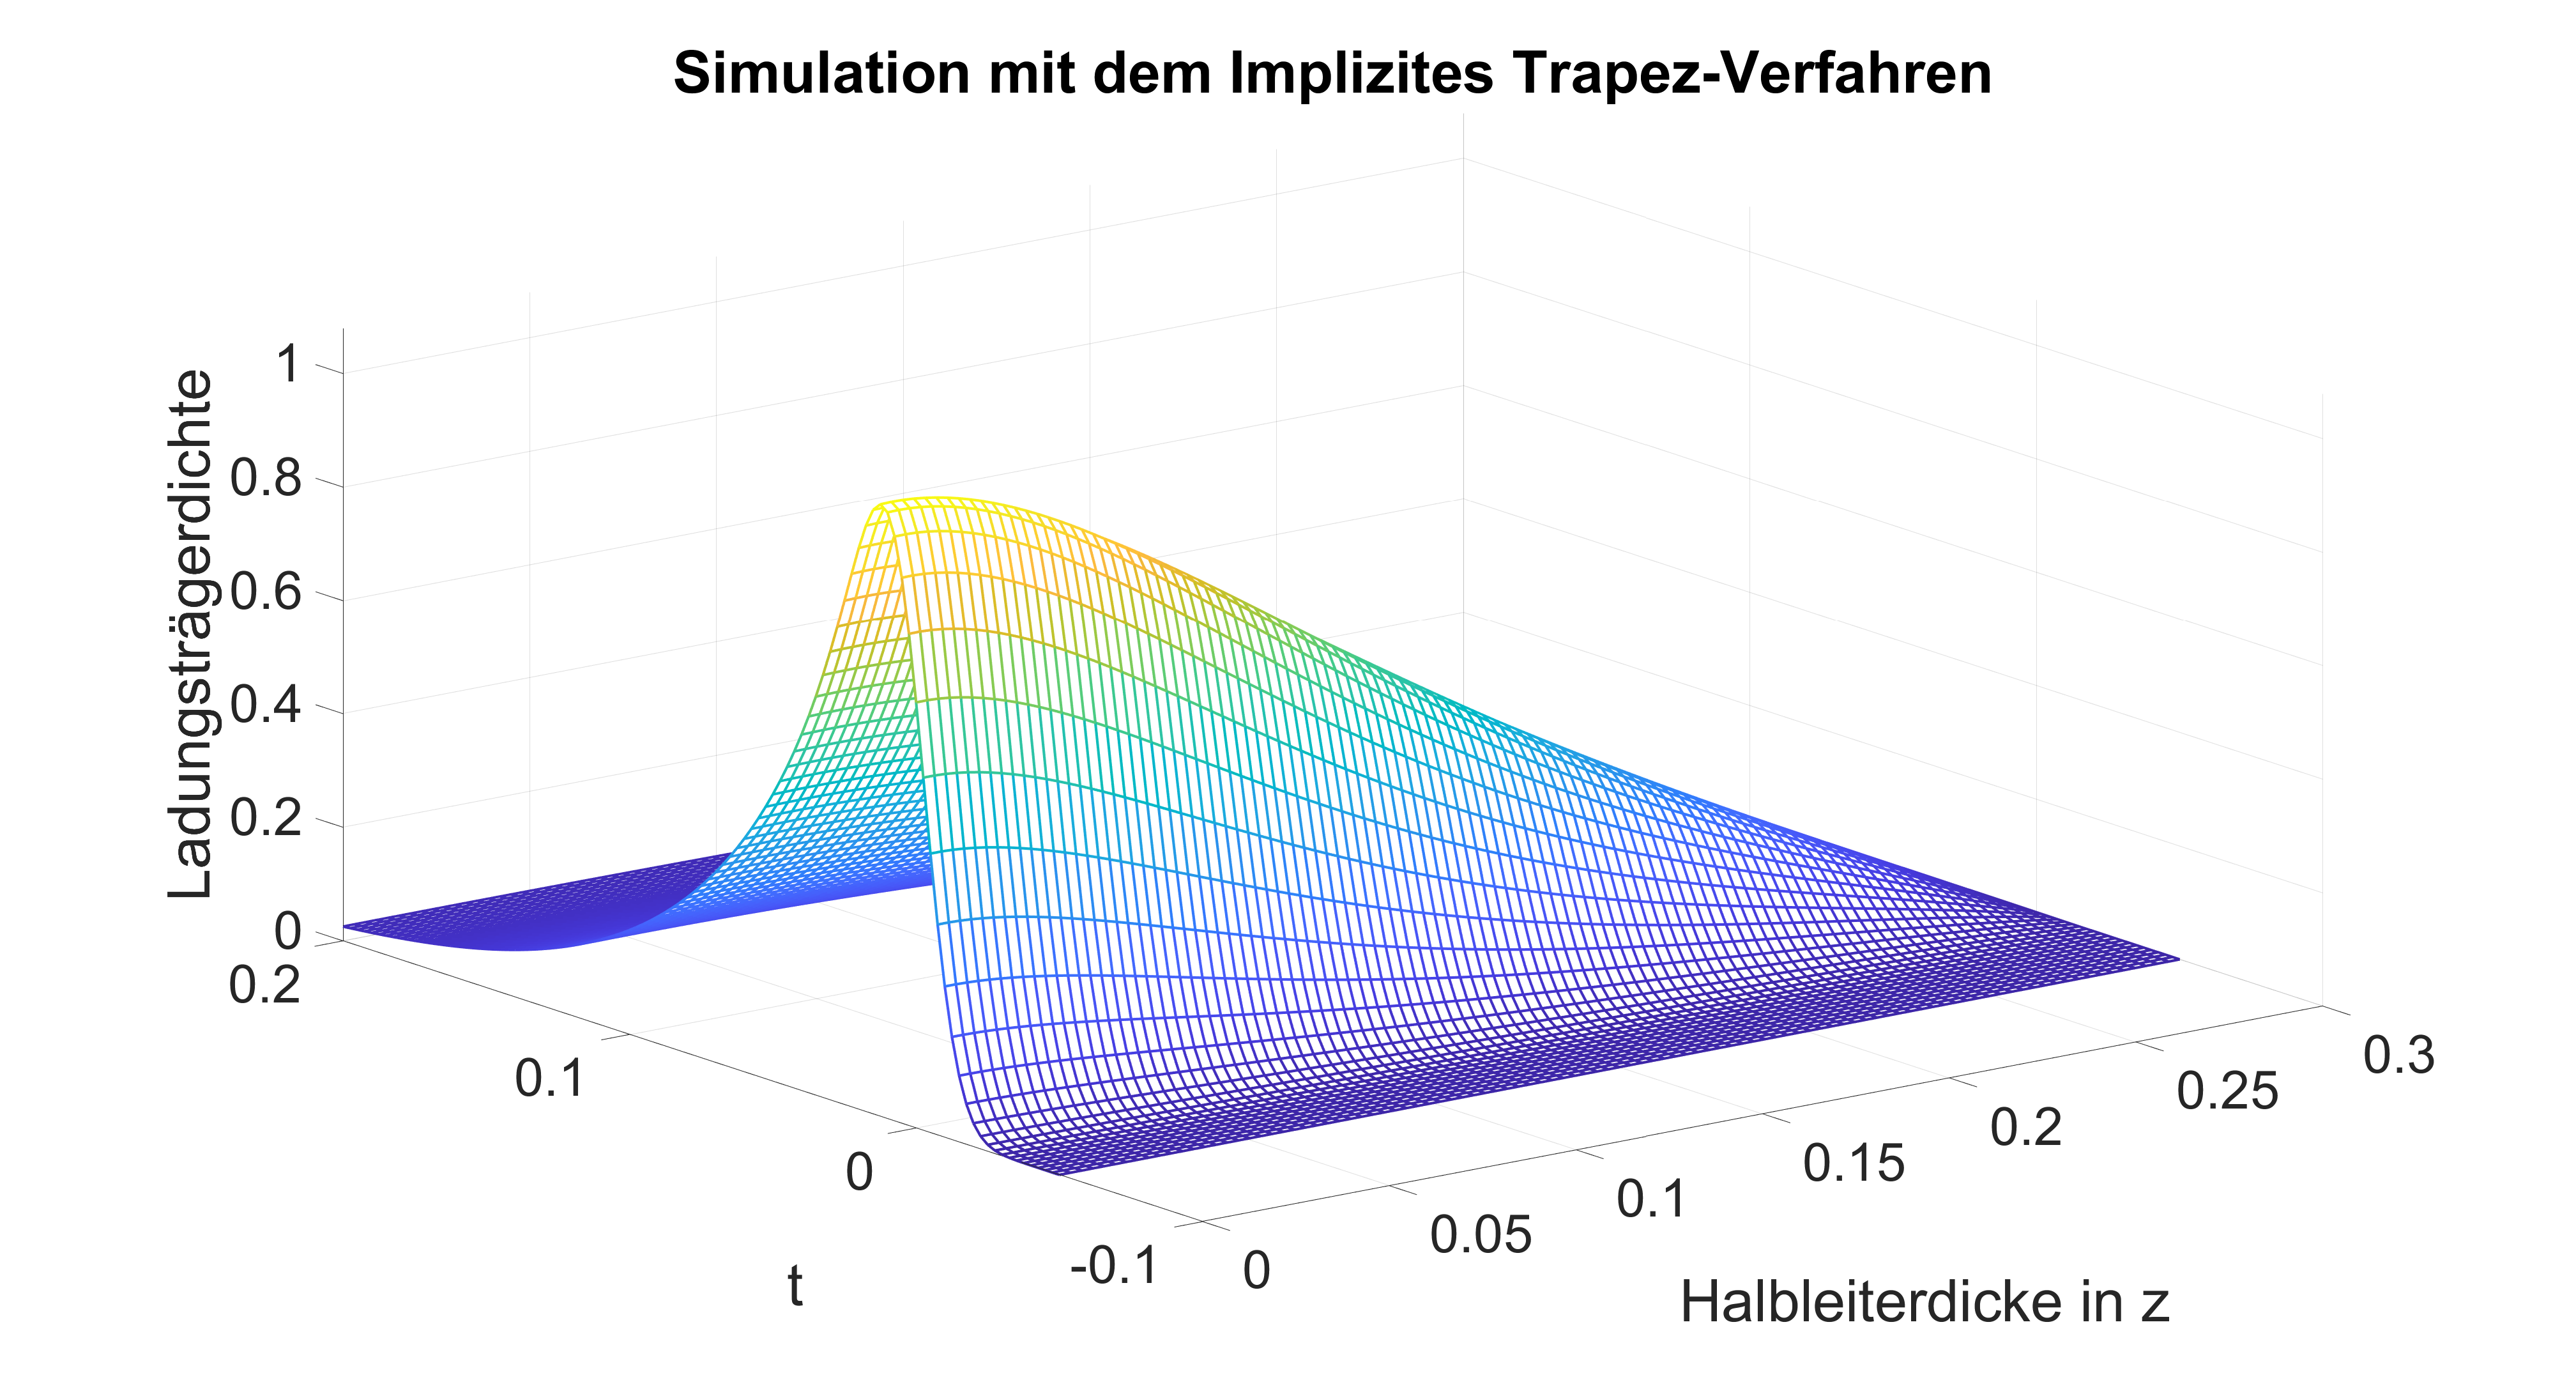
\includegraphics[width=1\linewidth]{figures/zeitaufgeloeste/S0}
		\caption{Trapezverfahren}
		\label{fig:s0}
	\end{subfigure}
	\hfill
	\begin{subfigure}[b]{0.5\textwidth}
			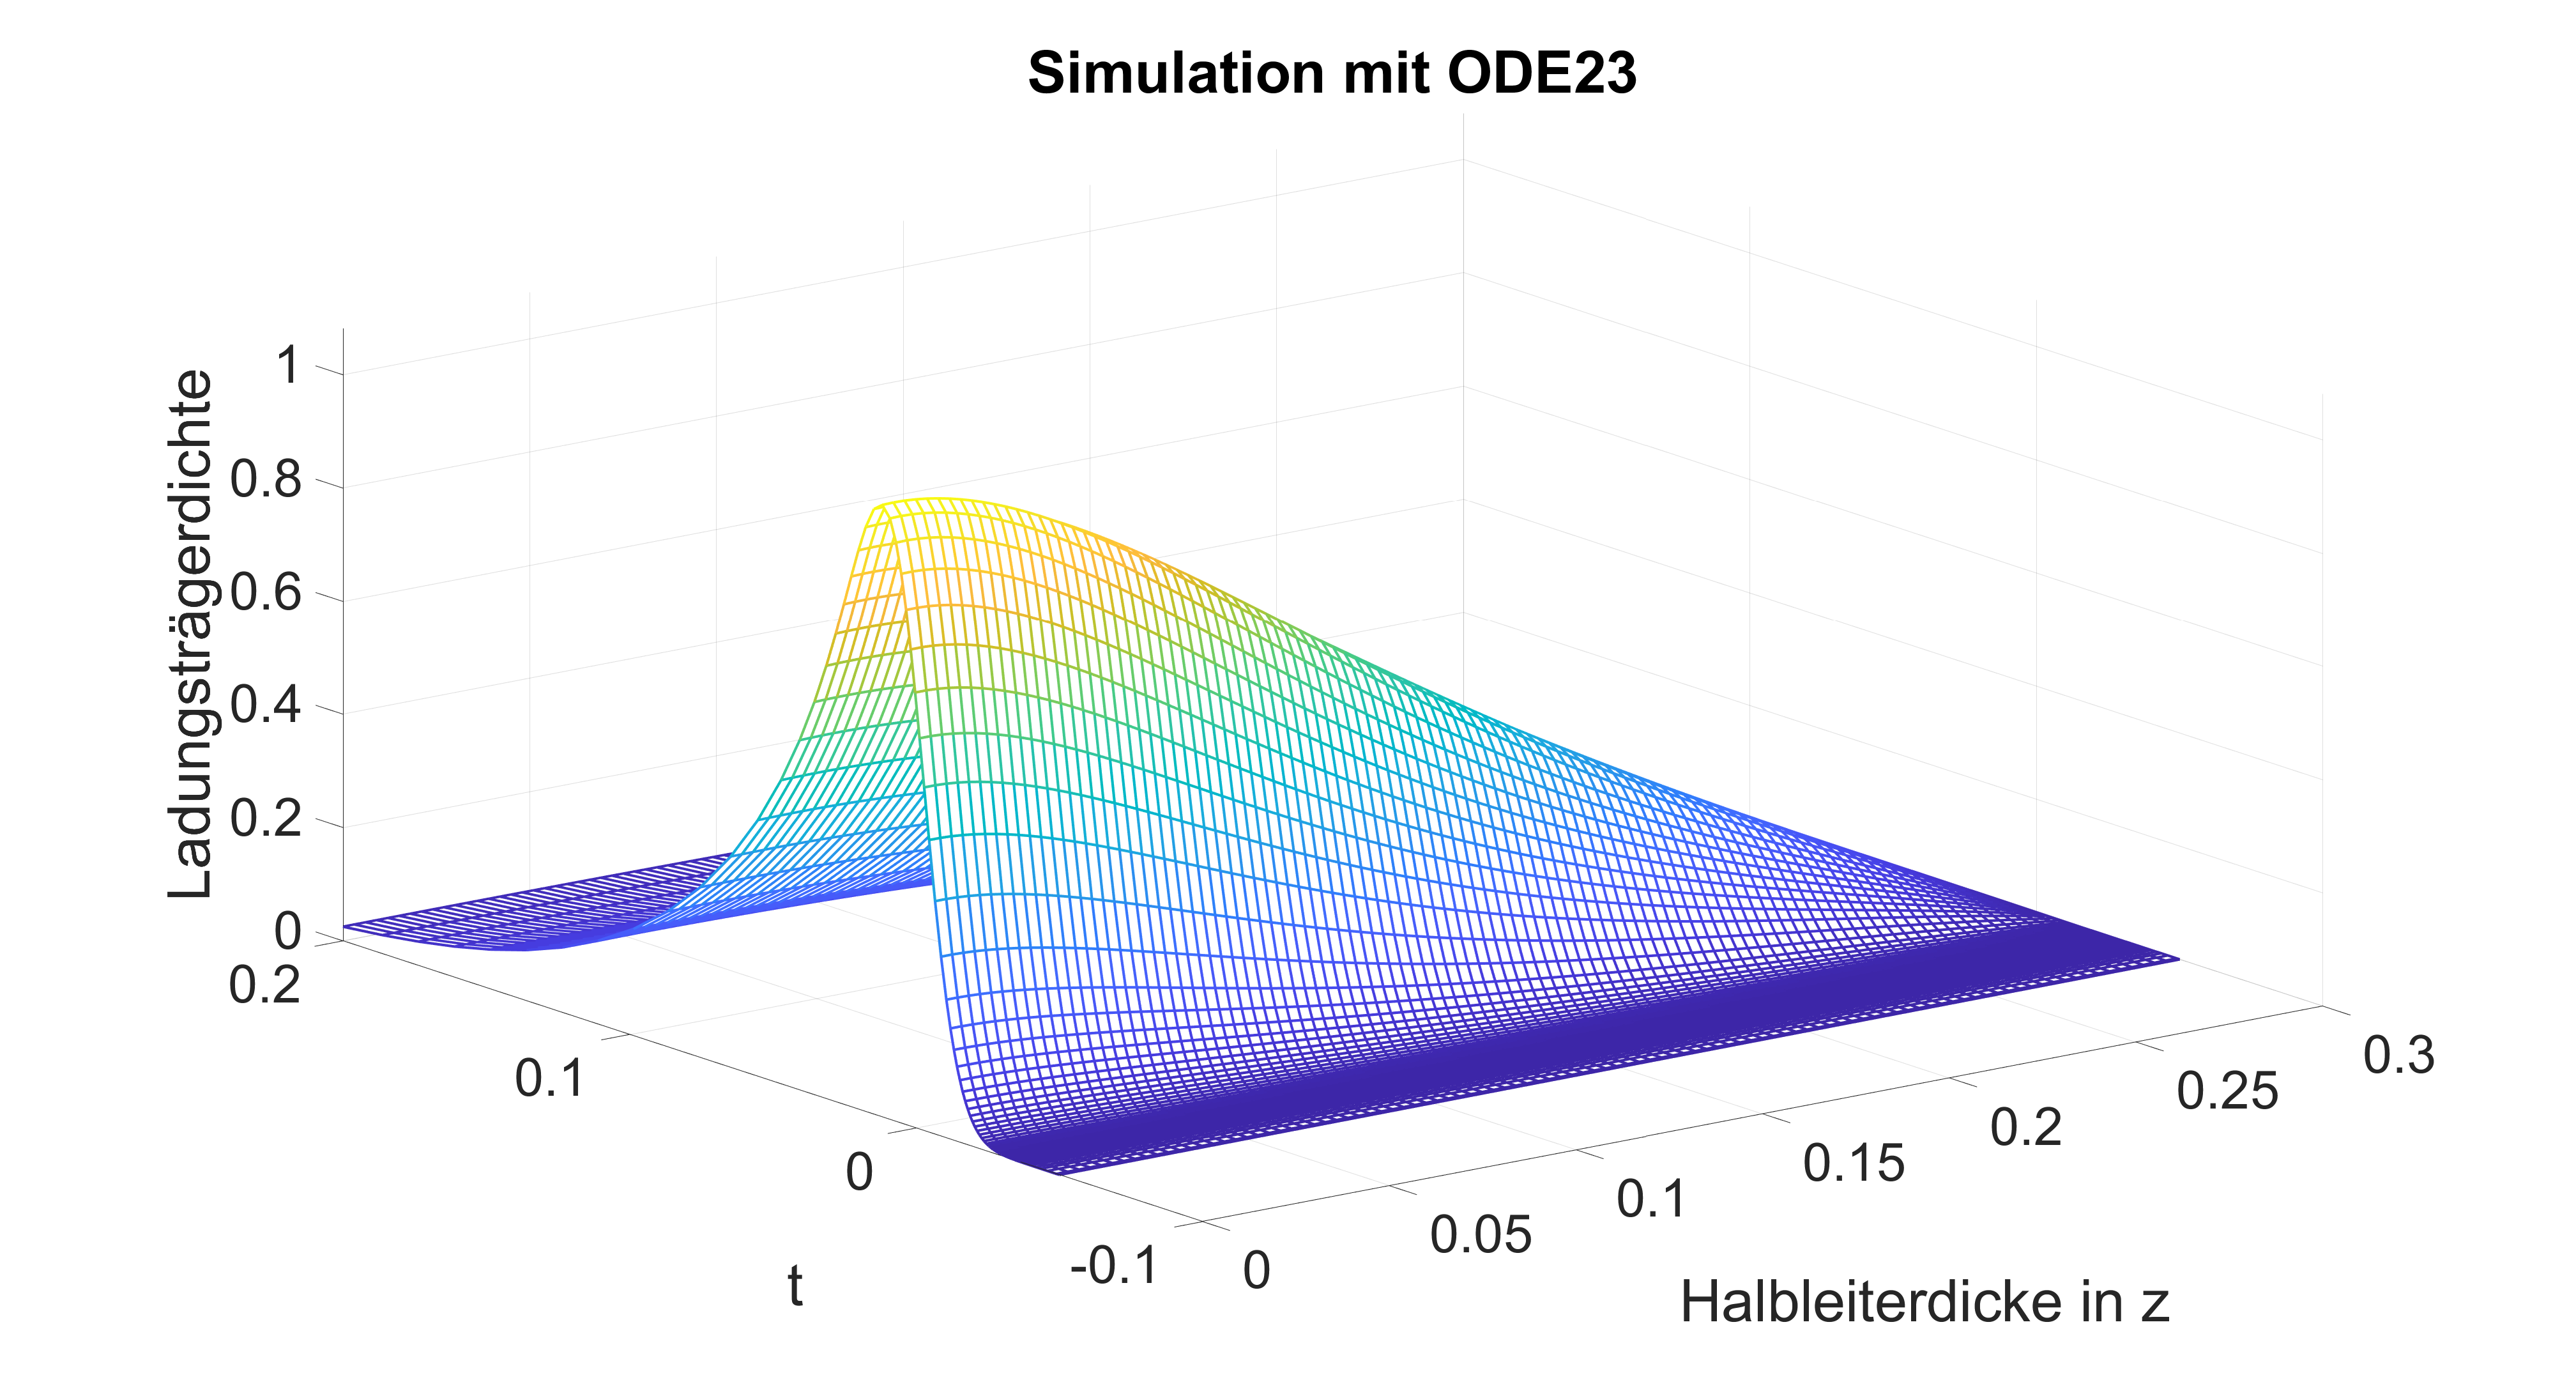
\includegraphics[width=1\linewidth]{figures/zeitaufgeloeste/S0_ode}
		\caption{ODE23}
		\label{fig:s0_ode}
	\end{subfigure}
	\caption{Auswertung der Zeitaufgelösten Simulation mit $S_0=10^4$ }
\end{figure}

\begin{figure}
	\centering

\end{figure}

\begin{figure}[h]
	
	\begin{subfigure}[b]{0.5\textwidth}
		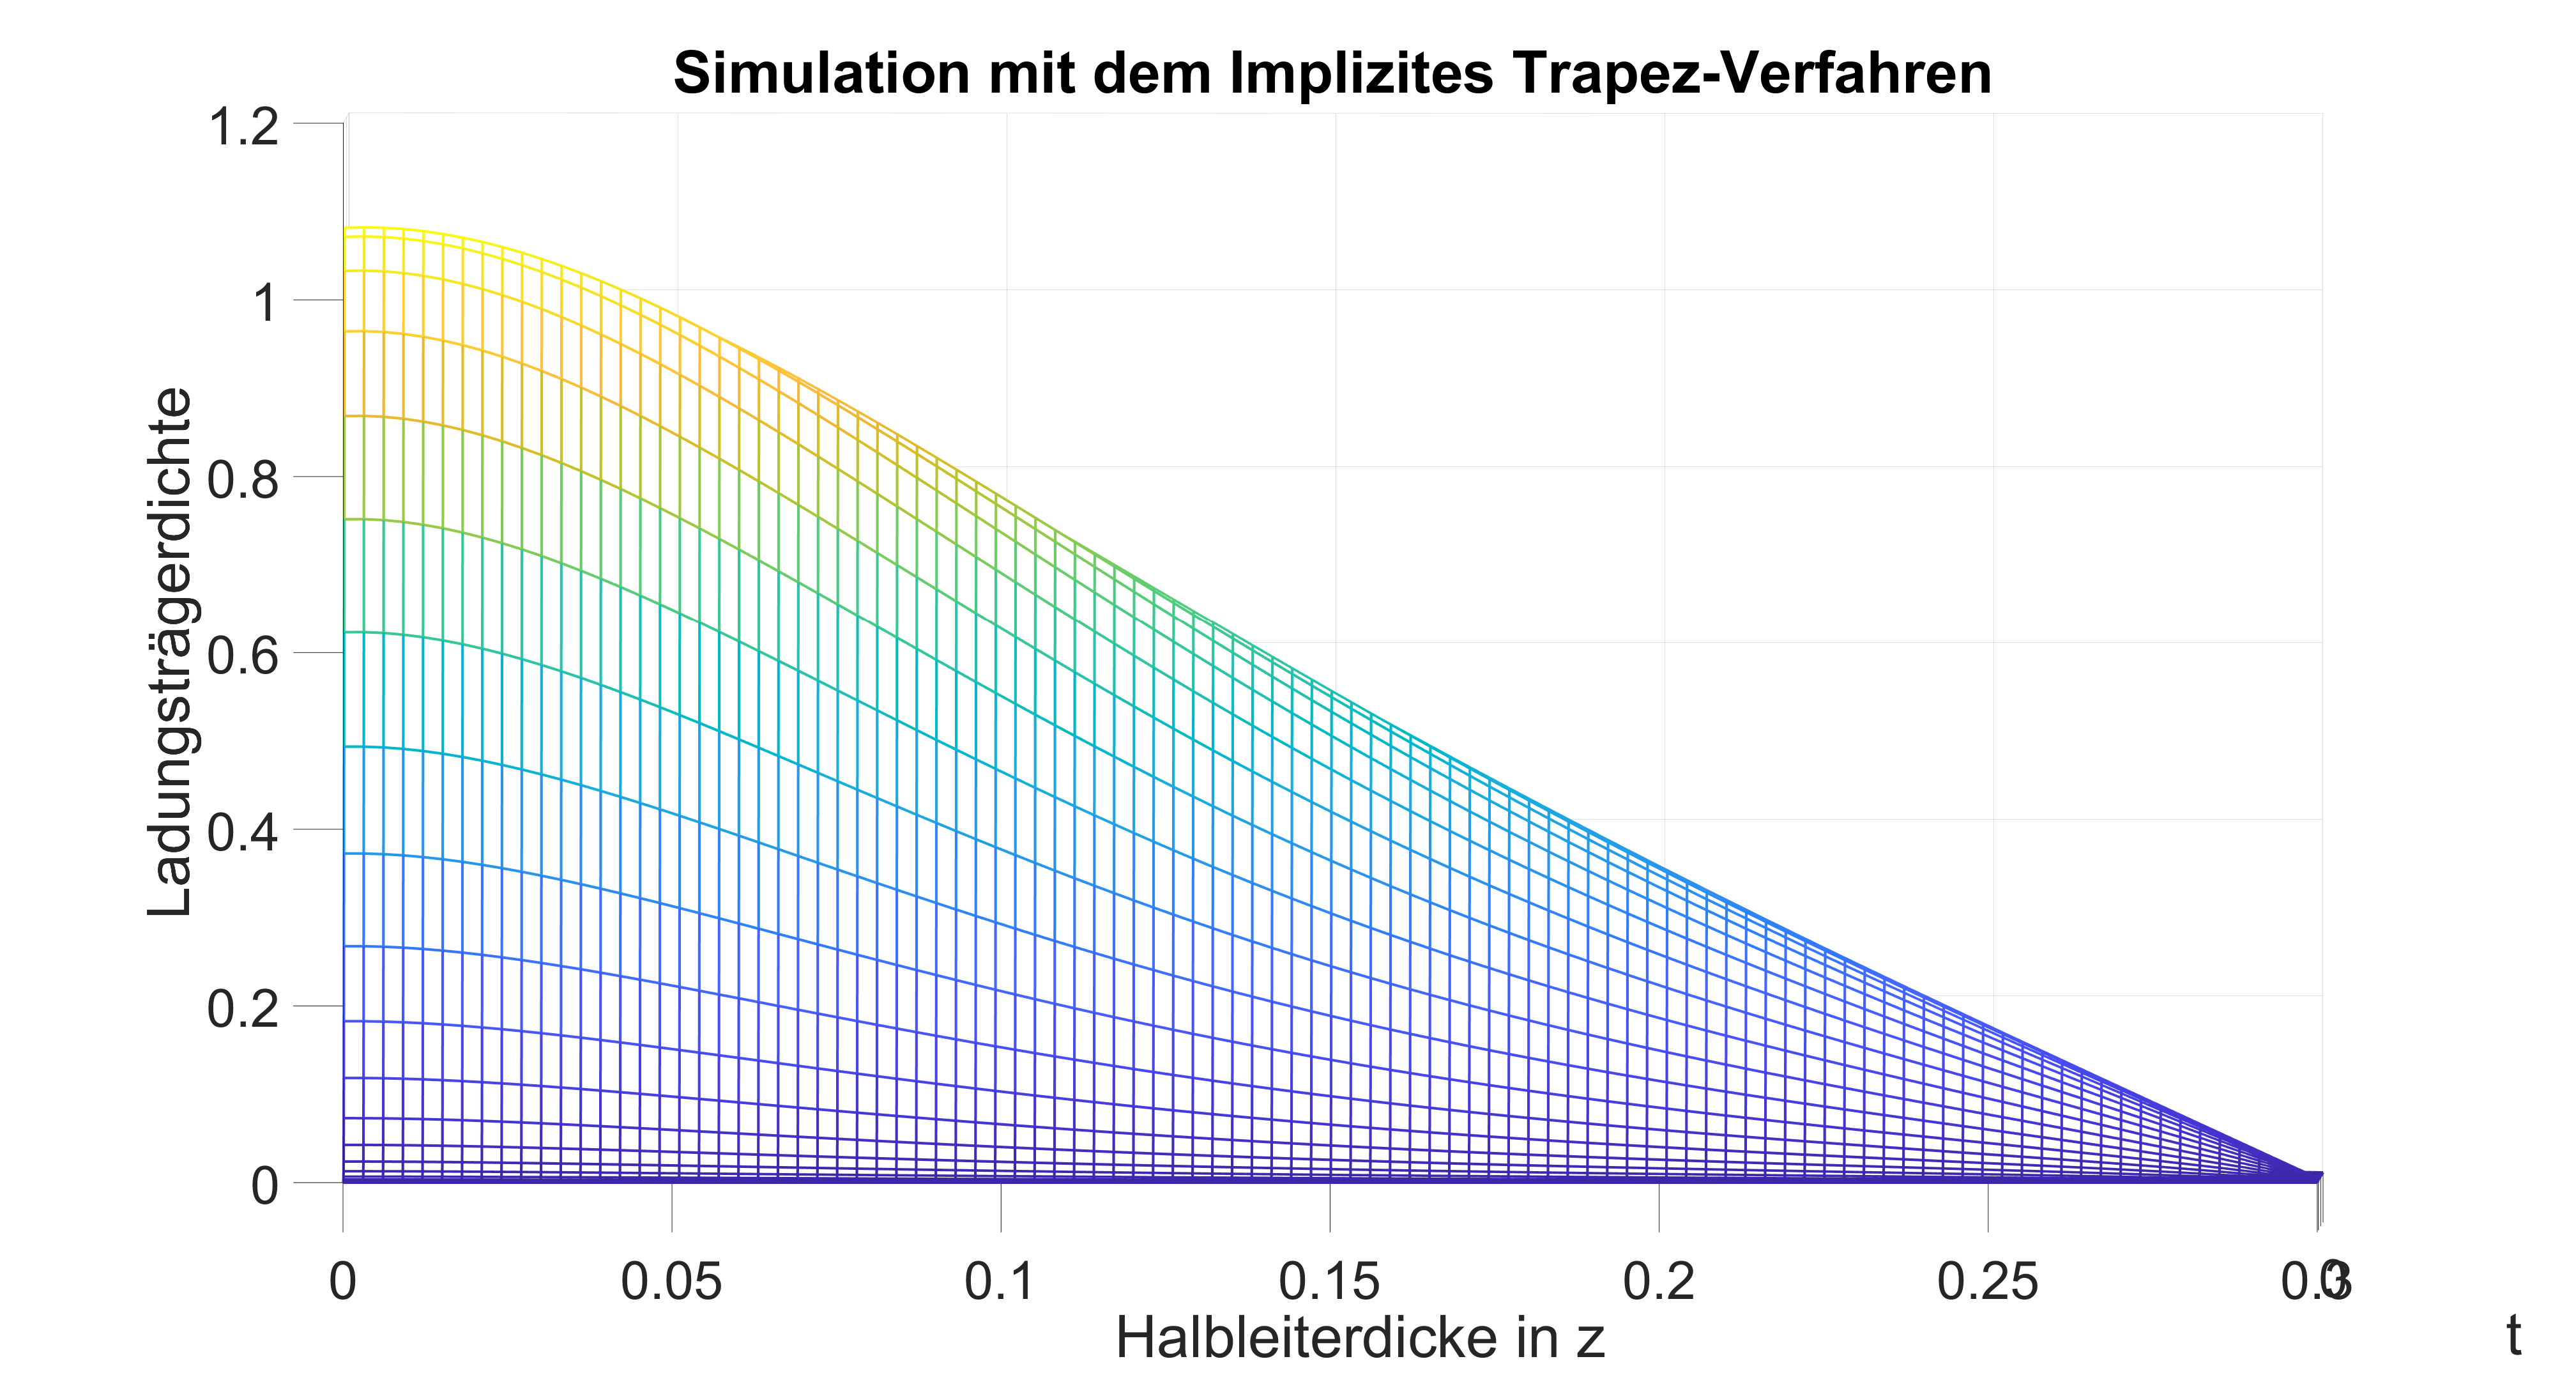
\includegraphics[width=1\linewidth]{figures/zeitaufgeloeste/S0_dicke}
	\caption{Betrachtung in $z$}
	\label{fig:s0dicke}
	\end{subfigure}
	\hfill
	\begin{subfigure}[b]{0.5\textwidth}
		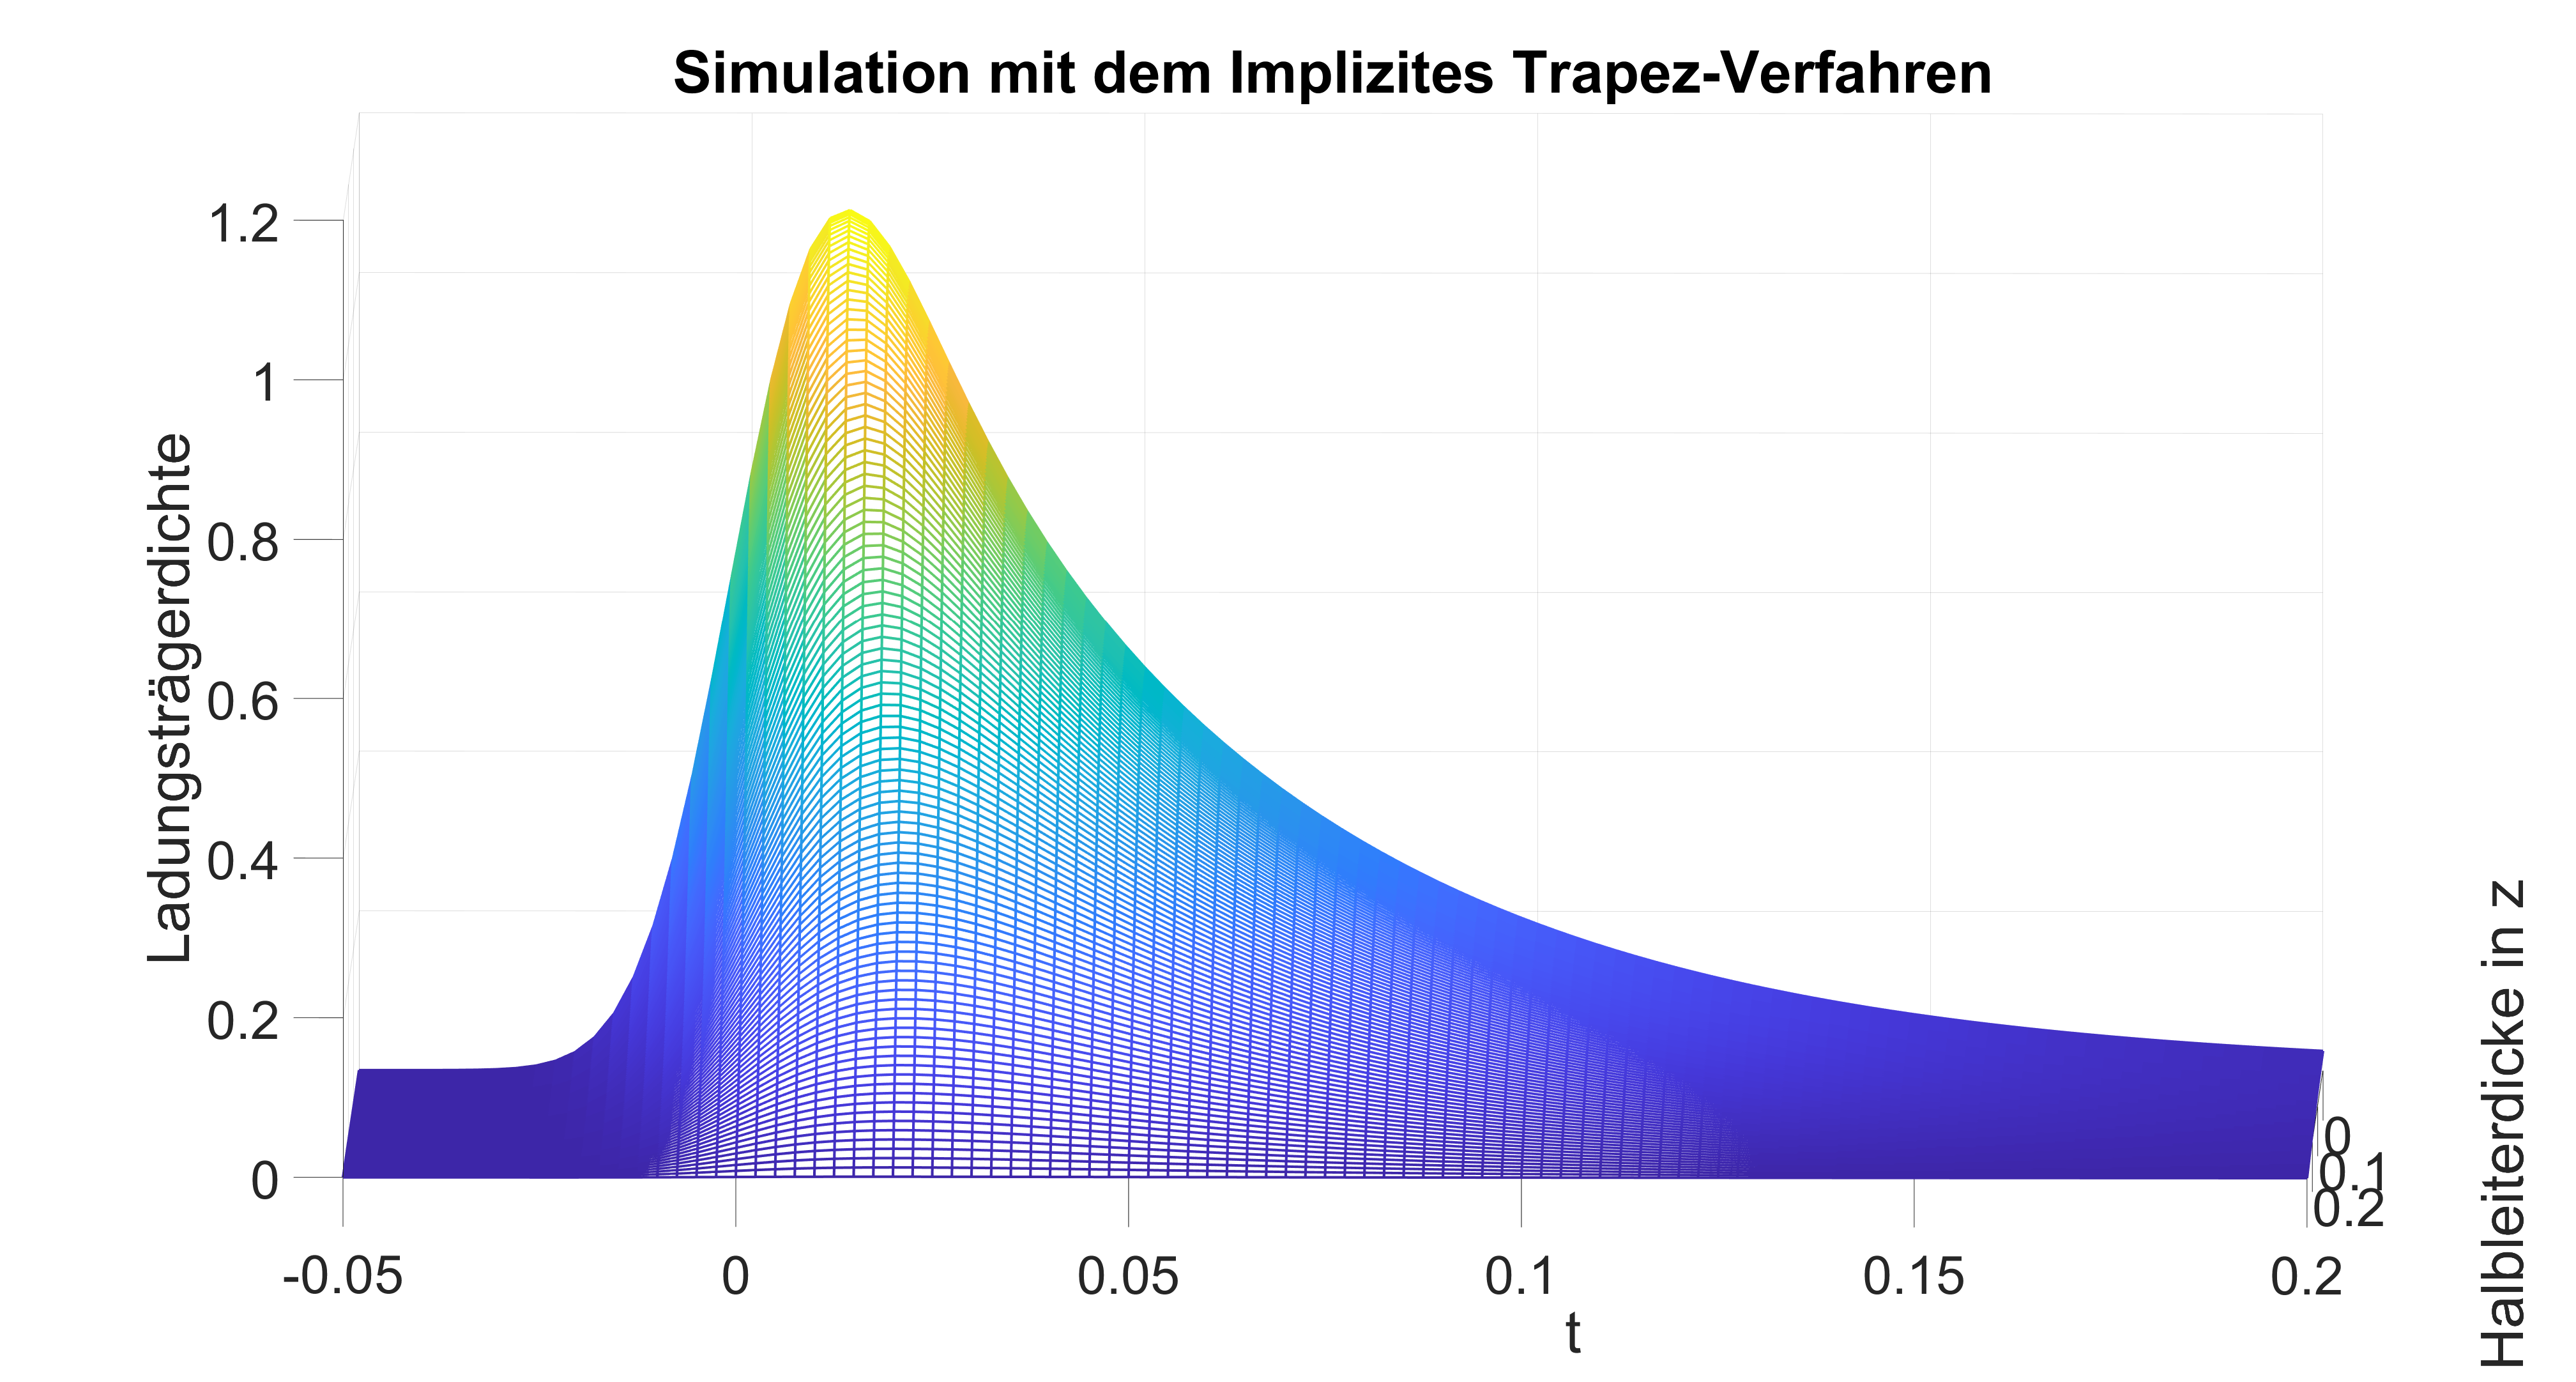
\includegraphics[width=1\linewidth]{figures/zeitaufgeloeste/S0_zeit}
		\caption{Betrachtung in $t$}
		\label{fig:s0_zeit}
	\end{subfigure}
	\caption{Vergleich von $z$ zu $t$}
\end{figure}
\begin{figure}[h]
	
	\begin{subfigure}[b]{0.5\textwidth}
		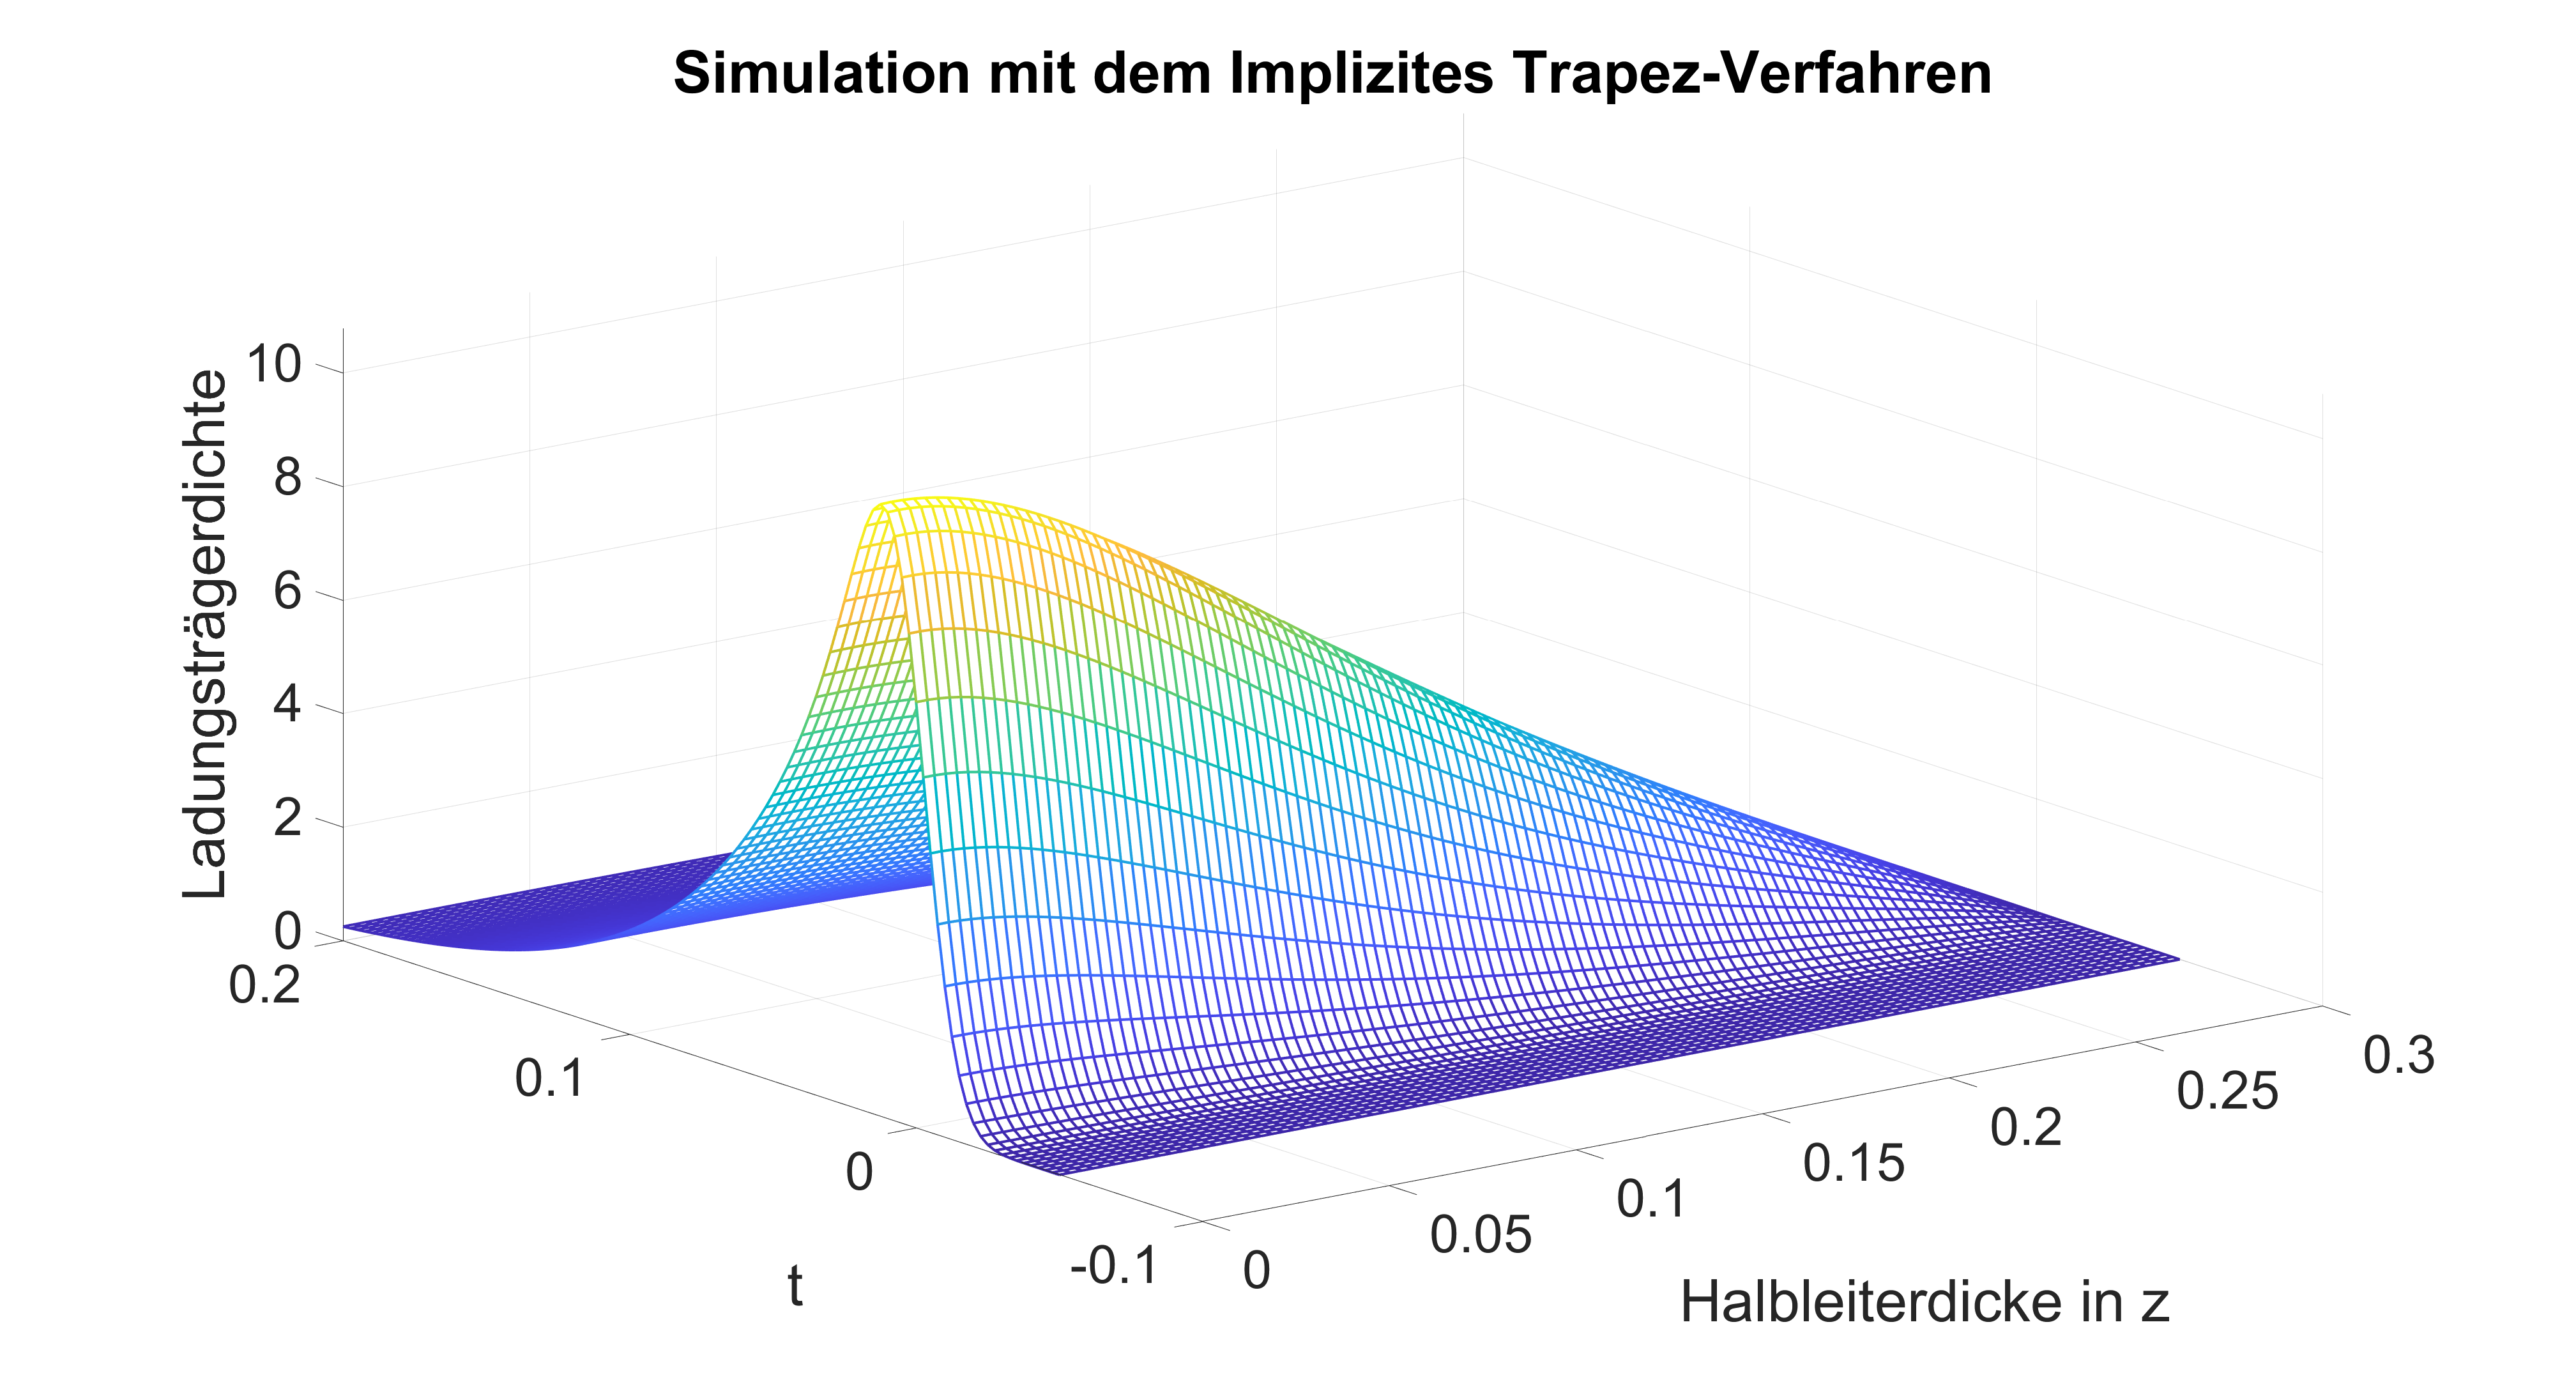
\includegraphics[width=1\linewidth]{figures/zeitaufgeloeste/S1}
		\caption{$S_0=10^5$}
		
	\end{subfigure}
	\hfill
	\begin{subfigure}[b]{0.5\textwidth}
		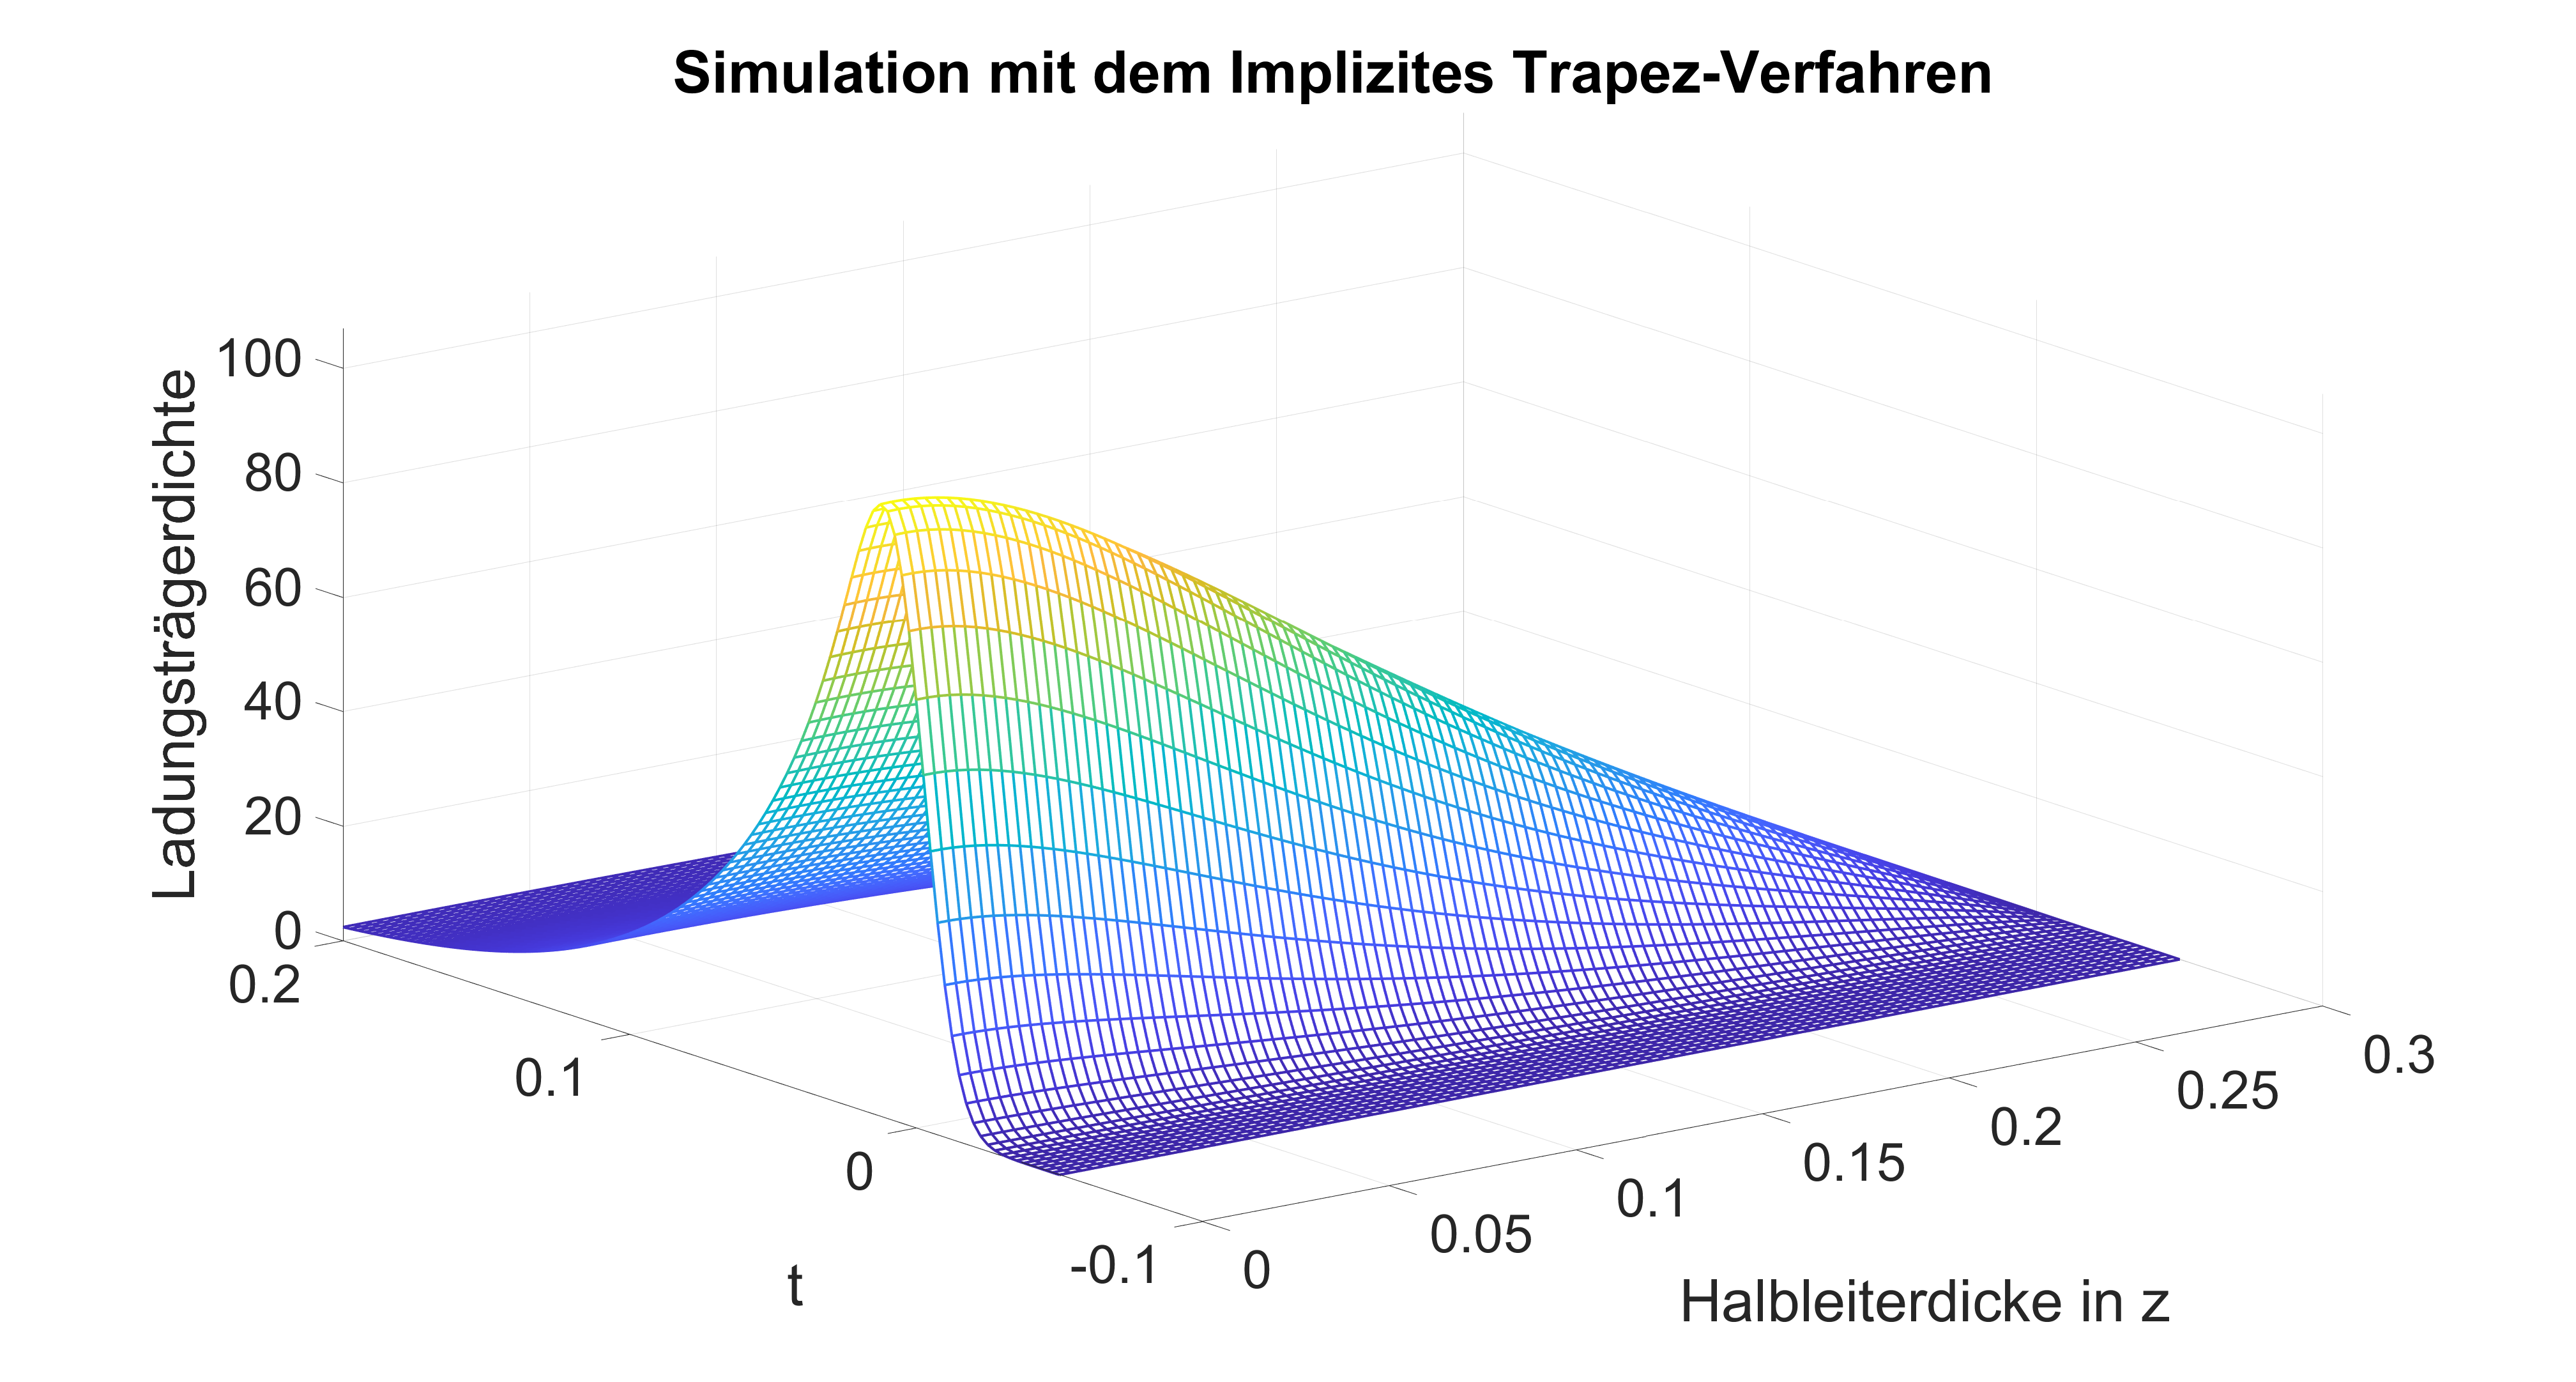
\includegraphics[width=1\linewidth]{figures/zeitaufgeloeste/S2}
		\caption{$S_0=10^6$}
	\end{subfigure}
	\caption{Auswertung der Zeitaufgelösten Simulation mit $S_0=10^5$ und $S_0=10^6$ }
\end{figure}
